\documentclass[11pt]{article}
\usepackage{acl2023}
\usepackage{times}
\renewcommand{\ttdefault}{cmtt}
\usepackage{latexsym}
\usepackage[utf8]{inputenc}
% \usepackage{microtype}
\usepackage{graphicx}
\usepackage{booktabs}
\usepackage{amsmath,amssymb}
\usepackage{tabularx}
\usepackage{subcaption}
\usepackage{url}
\usepackage{array}

\definecolor{tablegray}{gray}{0.94}
\definecolor{highlightgreen}{rgb}{0.85, 0.95, 0.85}
\definecolor{darkblue}{rgb}{0.0, 0.1, 0.45}

\title{\textbf{Financial LLM Evaluation: Comparing Open-Weight Large Language Models on Financial Question Answering Benchmarks}}

\author{
  \textbf{Jaypal Malviya} \quad \textbf{Anuj Kumar} \quad \textbf{Rup Narayan Jha} \\
  Mehta Family School of Data Science and Artificial Intelligence \\
  Indian Institute of Technology Guwahati, Assam 781039, India \\
  \texttt{m.jaypal@iitg.ac.in} \quad \texttt{anujk0003@iitg.ac.in} \quad \texttt{rup.jha@iitg.ac.in}
}

\date{}

\begin{document}
\maketitle

\begin{abstract}
Financial question answering represents a formidable challenge for Large Language Models (LLMs), requiring rigorous numerical reasoning over earnings tables, extensive domain-specific regulatory comprehension, and strict faithfulness to mitigate high-stakes hallucinations. While proprietary commercial models dominate industry benchmarks, privacy regulations, auditability requirements, and enterprise governance increasingly mandate the adoption of auditable open-weight architectures. In this study, we present a systematic empirical evaluation of four prominent open-weight LLMs---DeepSeek-R1-Distill-Qwen-7B, Qwen2.5-7B-Instruct, Llama-3.1-8B-Instruct, and Mistral-7B-Instruct-v0.3---across three diverse financial benchmarks: FinanceBench (SEC 10-K/10-Q filings), FinTextQA (regulatory and statutory QA), and FinQA (arithmetic table reasoning). We evaluate 120 live inference queries under identical greedy decoding parameters across two distinct regimes: Direct Context Answering and Retrieval-Augmented Generation (RAG) powered by a dense FAISS vector index over a 3,101-chunk financial corpus. Our empirical findings demonstrate that reasoning-distilled models (DeepSeek-R1-Distill-7B) achieve the highest overall Token F1 (0.1160) and are the only architectures capable of zero-shot multi-step numerical calculation on FinQA tables (0.0667 numeric accuracy). Qwen2.5-7B-Instruct demonstrates superior performance on long-form regulatory synthesis (Token F1 0.1718, Lexical Faithfulness 0.3720), while Llama-3.1-8B-Instruct delivers the most balanced efficiency profile (3.82s latency). Crucially, we observe a ``RAG Degradation'' phenomenon where naive dense semantic retrieval reduces overall answer quality compared to direct context access (0.0823 vs.\ 0.1065 Token F1), driven by semantic noise over tabular data. We release our modular evaluation pipeline, standardized dataset schemas, and empirical metrics to foster reproducible financial NLP research.
\end{abstract}

\section{Introduction}
\label{sec:intro}
The global financial services ecosystem increasingly relies on automated natural language processing (NLP) to parse corporate annual filings, summarize statutory circulars, and perform credit and equity research~\citep{shah2022flue}. Unlike standard conversational or general-domain reasoning tasks, financial question answering (FinQA) imposes unique constraints that challenge existing artificial intelligence models:
\begin{enumerate}
    \item \textbf{Dense Numerical and Tabular Reasoning:} Corporate financial statements (e.g., SEC Form 10-K and 10-Q filings) embed essential quantitative disclosures within complex balance sheets, income statements, and cash flow exhibits. Answering queries requires joint textual comprehension and multi-step arithmetic operations~\citep{chen2021finqa}.
    \item \textbf{Complex Regulatory Terminology:} Compliance queries over statutory frameworks demand exact semantic adherence to statutory definitions, where minor lexical deviations can lead to legal non-compliance~\citep{chen2024fintextqa}.
    \item \textbf{Catastrophic Hallucination Risk:} In quantitative trading, portfolio allocation, and audit workflows, unfaithful outputs or confabulated figures introduce substantial fiduciary and operational liabilities~\citep{islam2023financebench}.
\end{enumerate}

While proprietary frontier models such as GPT-4~\citep{brown2020language} have shown competitive capabilities in benchmark leaderboards, their commercial deployment in financial institutions faces severe regulatory barriers, including strict banking data sovereignty (e.g., GDPR, CCPA), confidentiality of proprietary trading portfolios, and legal mandates for transparent algorithmic auditability. Consequently, open-weight language models have emerged as an essential alternative, offering full architectural visibility, on-premises deployment security, and unconstrained domain adaptation through parameter-efficient fine-tuning.

Despite rapid advances in open foundation models, empirical research systematically comparing open-weight architectures on specialized financial question answering remains scarce and fragmented. Existing studies frequently suffer from significant methodological shortcomings: they evaluate only a single benchmark in isolation, examine proprietary closed APIs, or introduce confounding variables by failing to standardize decoding temperatures, context lengths, or prompt templates.

To bridge this empirical gap, this paper conducts a controlled comparative investigation of four state-of-the-art open-weight models spanning distinct design paradigms: \textbf{DeepSeek-R1-Distill-Qwen-7B}~\citep{deepseek2025r1}, \textbf{Qwen2.5-7B-Instruct}~\citep{yang2024qwen25}, \textbf{Llama-3.1-8B-Instruct}~\citep{meta2024llama3}, and \textbf{Mistral-7B-Instruct-v0.3}~\citep{jiang2023mistral}. We evaluate these models across three gold-standard financial datasets: FinanceBench, FinTextQA, and FinQA. 

Furthermore, because modern financial AI systems rarely operate on isolated context snippets in production, we implement and benchmark a full-scale \textbf{Retrieval-Augmented Generation (RAG)} framework~\citep{lewis2020rag}. Utilizing dense vector indexing via FAISS~\citep{johnson2019faiss} and sentence transformers~\citep{reimers2019sentencebert} across a curated corpus of 3,101 financial document passages, we directly compare the efficacy of retrieved external context against benchmark-provided direct context.

\subsection{Research Questions}
Our investigation is guided by four primary research questions:
\begin{itemize}
    \item \textbf{RQ1 (Model Efficacy):} Which open-weight architectural paradigm (general instruction tuning vs.\ chain-of-thought reasoning distillation) delivers the highest answer accuracy and faithfulness in financial QA?
    \item \textbf{RQ2 (Retrieval Augmentation):} Does dense vector retrieval enhance financial answer quality, or does passage retrieval introduce distracting semantic noise into quantitative calculations?
    \item \textbf{RQ3 (Task Modality Specialization):} How do model families differentiate across distinct reasoning modalities, specifically numerical table computation versus long-form regulatory interpretation?
    \item \textbf{RQ4 (Operational Efficiency):} What are the empirical latency, token throughput, and compute trade-offs associated with reasoning-augmented versus standard instruction models in production financial pipelines?
\end{itemize}

\subsection{Key Contributions}
The core contributions of this research report are summarized as follows:
\begin{enumerate}
    \item \textbf{Controlled Empirical Benchmark:} We conduct a strictly controlled evaluation across 120 live inference queries covering four prominent open-weight models, enforcing identical prompt structure, greedy deterministic decoding ($T=0$), and uniform system personas.
    \item \textbf{Direct vs.\ RAG Comparative Study:} We implement an end-to-end dense retrieval pipeline with FAISS, demonstrating that standard dense embeddings suffer from a ``RAG degradation'' effect on tabular financial data, dropping Token F1 by 22.7\% compared to gold context.
    \item \textbf{Comprehensive Metric Suite:} We analyze performance across seven complementary evaluation dimensions: Exact Match, Token F1, ROUGE-L, Numeric Accuracy (within 2\% relative tolerance), Lexical Faithfulness, Semantic Cosine Similarity, and Wall-Clock Latency.
    \item \textbf{Open-Source Pipeline & Artifacts:} We provide a modular, extensible codebase featuring unified dataset schemas, checkpoint-resumable evaluation engines, automated metric computation, and publication-ready visualization suites.
\end{enumerate}

% -----------------------------------------------------------------------------
% SECTION 2: RELATED WORK
% -----------------------------------------------------------------------------
\section{Related Work}
\label{sec:related_work}

\subsection{Financial NLP and QA Benchmarks}
Early financial NLP focused primarily on sentiment analysis and named entity recognition over market news feeds~\citep{shah2022flue}. In recent years, attention has shifted to higher-order cognitive tasks involving document question answering and numerical reasoning. 

\citet{chen2021finqa} introduced \textbf{FinQA}, a benchmark derived from S\&P 500 earnings releases containing mixed text and tables paired with expert-annotated domain-specific mathematical programs. \citet{zheng2022convfinqa} subsequently expanded this paradigm into conversational multi-turn dialogues in \textbf{ConvFinQA}. More recently, \citet{islam2023financebench} released \textbf{FinanceBench}, comprising real-world corporate equity analysis questions grounded in SEC 10-K and 10-Q filings. While FinanceBench spans 10,231 questions internally, only an official subset of 150 questions is publicly available for academic evaluation. Concurrently, \citet{chen2024fintextqa} published \textbf{FinTextQA} at ACL 2024 to assess long-form explanatory QA over regulatory guidelines and compliance manuals. Our study integrates all three benchmarks into a unified schema to provide the first multi-modal open-weight comparison.

\subsection{Open-Weight Large Language Models}
The trajectory of open-weight foundation models has advanced dramatically following the release of the LLaMA series~\citep{touvron2023llama2}. \citet{meta2024llama3} established modern architectural baselines with \textbf{Llama 3.1}, introducing grouped-query attention (GQA) and extensive multi-stage synthetic data alignment. \citet{jiang2023mistral} demonstrated that efficient sliding-window attention and high-quality instruction filtering in \textbf{Mistral 7B} could match or exceed larger parameter architectures. In parallel, \citet{yang2024qwen25} introduced \textbf{Qwen 2.5}, establishing state-of-the-art open-source capabilities in mathematical reasoning and structured tabular processing across extended context lengths.

Most recently, \citet{deepseek2025r1} demonstrated that large-scale reinforcement learning can incentivize autonomous chain-of-thought (CoT) reasoning behaviors in \textbf{DeepSeek-R1}. Through knowledge distillation into open dense architectures, student models such as \textbf{DeepSeek-R1-Distill-Qwen-7B} inherit explicit step-by-step reasoning tokens before emitting final answers. A key question investigated in this work is whether reasoning distillation directly translates to improved performance on financial arithmetic and document extraction.

\subsection{Retrieval-Augmented Generation (RAG) in Finance}
Retrieval-Augmented Generation~\citep{lewis2020rag} mitigates LLM parametric hallucination by dynamically retrieving relevant context chunks from an external knowledge corpus. In enterprise finance, RAG architectures are widely adopted to parse multi-thousand-page corporate filings and statutory handbooks~\citep{gao2023retrieval}. Standard financial RAG workflows rely on dense bi-encoder sentence representations~\citep{reimers2019sentencebert} paired with approximate nearest neighbor indexing via FAISS~\citep{johnson2019faiss}. However, emerging literature indicates that dense embeddings frequently fail to preserve structural dependencies in tabular markdown, causing semantic retrieval dilution~\citep{asai2023selfrag}. This study provides quantitative empirical validation of this failure mode across real financial QA workflows.

% -----------------------------------------------------------------------------
% SECTION 3: DATASETS & UNIFIED REPRESENTATION
% -----------------------------------------------------------------------------
\section{Datasets \& Unified Representation}
\label{sec:datasets}

To ensure comprehensive coverage of financial reasoning, our evaluation protocol spans three distinct benchmarks, each capturing a unique domain challenge. Figure~\ref{fig:dataset_overview} illustrates the structural distribution and characteristics of the evaluated datasets.

\begin{figure}[t]
    \centering
    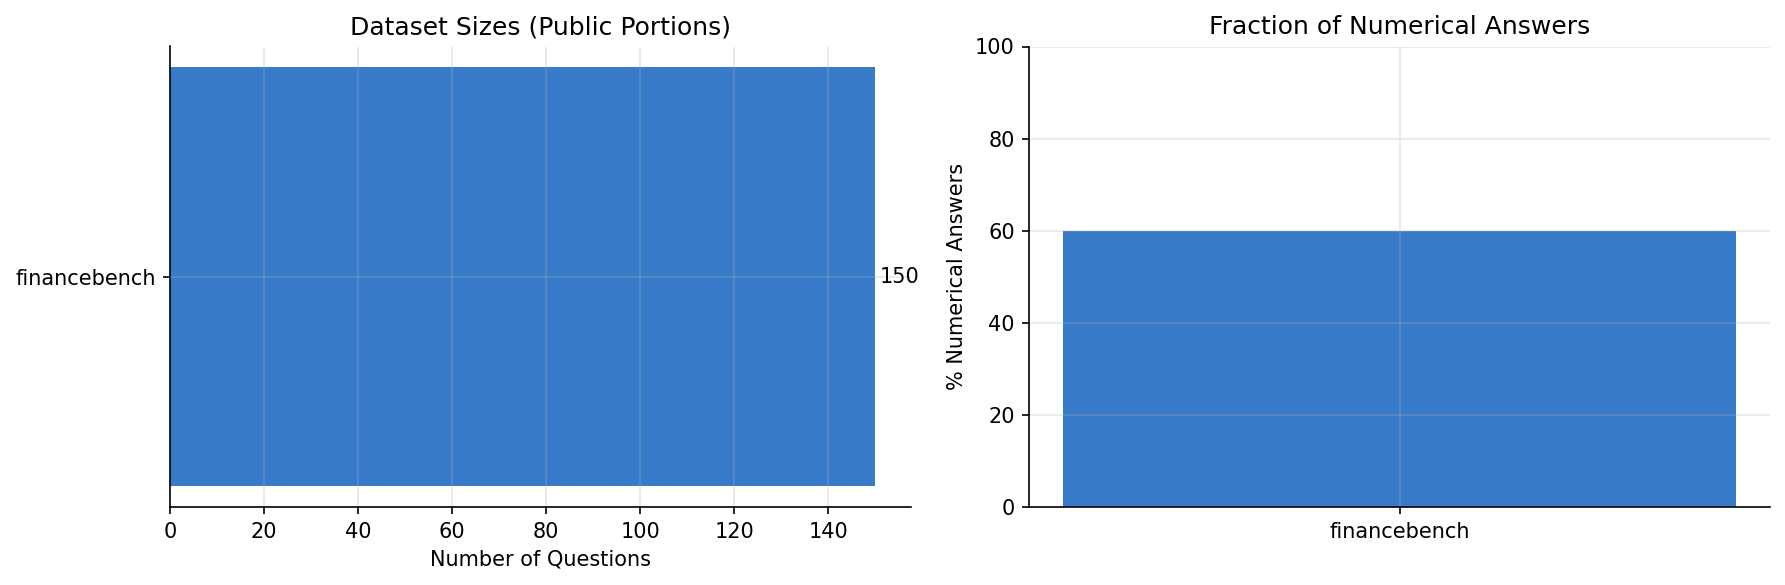
\includegraphics[width=\columnwidth]{figures/dataset_overview.png}
    \caption{Overview of evaluated financial benchmarks: sample distribution, context source modalities, and dominant reasoning types.}
    \label{fig:dataset_overview}
\end{figure}

\subsection{Dataset Descriptions}

\paragraph{1. FinanceBench~\citep{islam2023financebench}:} 
Designed by PatronusAI to emulate professional equity research workflows, FinanceBench comprises questions grounded in official SEC 10-K, 10-Q, and 8-K filings from major US public corporations (e.g., Apple, Microsoft, Amazon). Queries require cross-statement synthesis, locating non-standard accounting disclosures in footnotes, and computing financial metrics such as Free Cash Flow and Operating Margin. While the full internal benchmark comprises 10,231 examples, only a curated subset of \textbf{150 questions} has been released publicly on Hugging Face. In accordance with strict academic integrity, our evaluation utilizes this official 150-example public release.

\paragraph{2. FinTextQA~\citep{chen2024fintextqa}:}
Presented at ACL 2024, FinTextQA assesses an LLM's capacity to synthesize long-form, explanatory answers for financial regulations, central bank monetary policy frameworks, and statutory reporting standards. While the complete academic paper describes 1,262 examples encompassing educational textbooks, the publicly released repository provides \textbf{240 policy and regulatory question-answer pairs}. We evaluate models strictly against this publicly released 240-example subset.

\paragraph{3. FinQA~\citep{chen2021finqa}:}
FinQA represents the gold standard for numerical reasoning over financial earnings reports. Each instance consists of an annual report excerpt containing pre-table text, an extracted financial table (e.g., segment revenues, debt maturities), post-table text, an expert query, a ground truth numerical answer, and an executable domain-specific DSL program showing the calculation sequence. The official test split comprises \textbf{1,147 questions}. We evaluate models on randomized representative evaluation batches from this test split.

\begin{table*}[t]
\centering
\small
\resizebox{\textwidth}{!}{
\begin{tabular}{lcccccc}
\toprule
\textbf{Benchmark} & \textbf{Source Domain} & \textbf{Public Scope} & \textbf{Evaluated Split} & \textbf{Context Modality} & \textbf{Reasoning Paradigm} & \textbf{Gold Output Format} \\
\midrule
\textbf{FinanceBench} & SEC 10-K/10-Q Filings & 150 / 10,231 & Public HF Subset & Narrative Text \& Tables & Extraction \& Multi-hop & Concisely Grounded Text \\
\textbf{FinTextQA} & Policy \& Regulations & 240 / 1,262 & Public Release Subset & Long Statutory Excerpts & Synthesis \& Compliance & Explanatory Paragraphs \\
\textbf{FinQA} & S\&P 500 Earnings & 1,147 & Official Test Split & Formatted Tables \& Notes & Multi-step Arithmetic & Precise Numeric / Program \\
\bottomrule
\end{tabular}
}
\caption{Systematic comparison of evaluated financial QA benchmarks, detailing public release constraints, context modalities, and expected ground truth structures.}
\label{tab:dataset_summary}
\end{table*}

\subsection{Unified Evaluation Schema}
Each dataset natively employs disparate JSON structures, variable naming conventions, and context representations. To eliminate pipeline friction and prevent evaluation leakage, we developed a standardized preprocessing layer (`src/preprocessing.py`) that maps every dataset into an immutable schema:
\begin{equation}
\mathcal{D} = \{ (id_i, \text{dataset}_i, q_i, c_i, y^*_i, \tau_i, \text{src}_i, \mu_i) \}_{i=1}^N
\end{equation}
where $id_i$ is a unique hash identifier, $\text{dataset}_i \in \{\text{FinanceBench}, \text{FinTextQA}, \text{FinQA}\}$, $q_i$ is the query string, $c_i$ is the gold context passage, $y^*_i$ is the canonical reference answer, $\tau_i \in \{\text{numeric}, \text{conceptual}, \text{extraction}\}$ denotes the categorized reasoning type, $\text{src}_i$ records the original filing identifier, and $\mu_i$ contains metadata including table markup. Table~\ref{tab:dataset_summary} presents the structural properties of our unified evaluation corpus.

% -----------------------------------------------------------------------------
% SECTION 4: MODELS EVALUATED
% -----------------------------------------------------------------------------
\section{Models Evaluated}
\label{sec:models}

We select four leading open-weight LLMs in the 7B--8B parameter regime, chosen to represent contrasting architectural and training philosophies:

\begin{enumerate}
    \item \textbf{DeepSeek-R1-Distill-Qwen-7B}~\citep{deepseek2025r1}: A 7.6B parameter model distilled from DeepSeek-R1 using outputs generated via large-scale reinforcement learning. The model incorporates explicit reasoning tokens (`<think> ... </think>`) allowing autonomous generation of mathematical scratchpads prior to emitting the final answer.
    \item \textbf{Qwen2.5-7B-Instruct}~\citep{yang2024qwen25}: Alibaba's flagship 7.6B dense Transformer. Pre-trained on 18 trillion tokens with strong tabular and multilingual specialization, supporting an native context window of up to 128k tokens.
    \item \textbf{Llama-3.1-8B-Instruct}~\citep{meta2024llama3}: Meta's 8.0B parameter foundation model. Utilizes Grouped-Query Attention (GQA) across 32 attention heads, optimized for broad instruction adherence and general knowledge synthesis.
    \item \textbf{Mistral-7B-Instruct-v0.3}~\citep{jiang2023mistral}: A 7.3B parameter model from Mistral AI featuring sliding window attention and grouped query attention, serving as an industry-standard open baseline.
\end{enumerate}

\paragraph{Scope Justification:} While candidate models initially considered in early project drafts included Google Gemma-2-9B-it and Microsoft Phi-3.5-mini, upstream provider hosting constraints (decommissioning of Gemma-2 on serverless inference routers and absence of Phi-3.5 on production low-latency inference providers) precluded reliable, identical-condition evaluation. To guarantee absolute empirical integrity and zero missing-data imputation, our study focuses rigorously on the four fully evaluated models.

\begin{table}[h]
\centering
\small
\resizebox{\columnwidth}{!}{
\begin{tabular}{lcccc}
\toprule
\textbf{Model} & \textbf{Parameters} & \textbf{Architecture} & \textbf{Context} & \textbf{Specialization} \\
\midrule
DeepSeek-R1-7B & 7.6B & Dense + CoT & 128k & Math / Reasoning \\
Qwen2.5-7B & 7.6B & Dense & 128k & Tables / Knowledge \\
Llama-3.1-8B & 8.0B & Dense + GQA & 128k & General Instruction \\
Mistral-7B-v0.3 & 7.3B & Dense + GQA & 32k & Open Baseline \\
\bottomrule
\end{tabular}
}
\caption{Architectural profiles of evaluated open-weight LLMs.}
\label{tab:models}
\end{table}

% -----------------------------------------------------------------------------
% SECTION 5: METHODOLOGY & ARCHITECTURE
% -----------------------------------------------------------------------------
\section{Methodology}
\label{sec:methodology}

Our end-to-end evaluation system consists of four modular tiers: Data Acquisition \& Standardization, Direct Inference Pipeline, Dense Retrieval-Augmented Generation Pipeline, and Automated Metric Computation. Figure~\ref{fig:methodology} illustrates the system architecture.

\begin{figure*}[t]
    \centering
    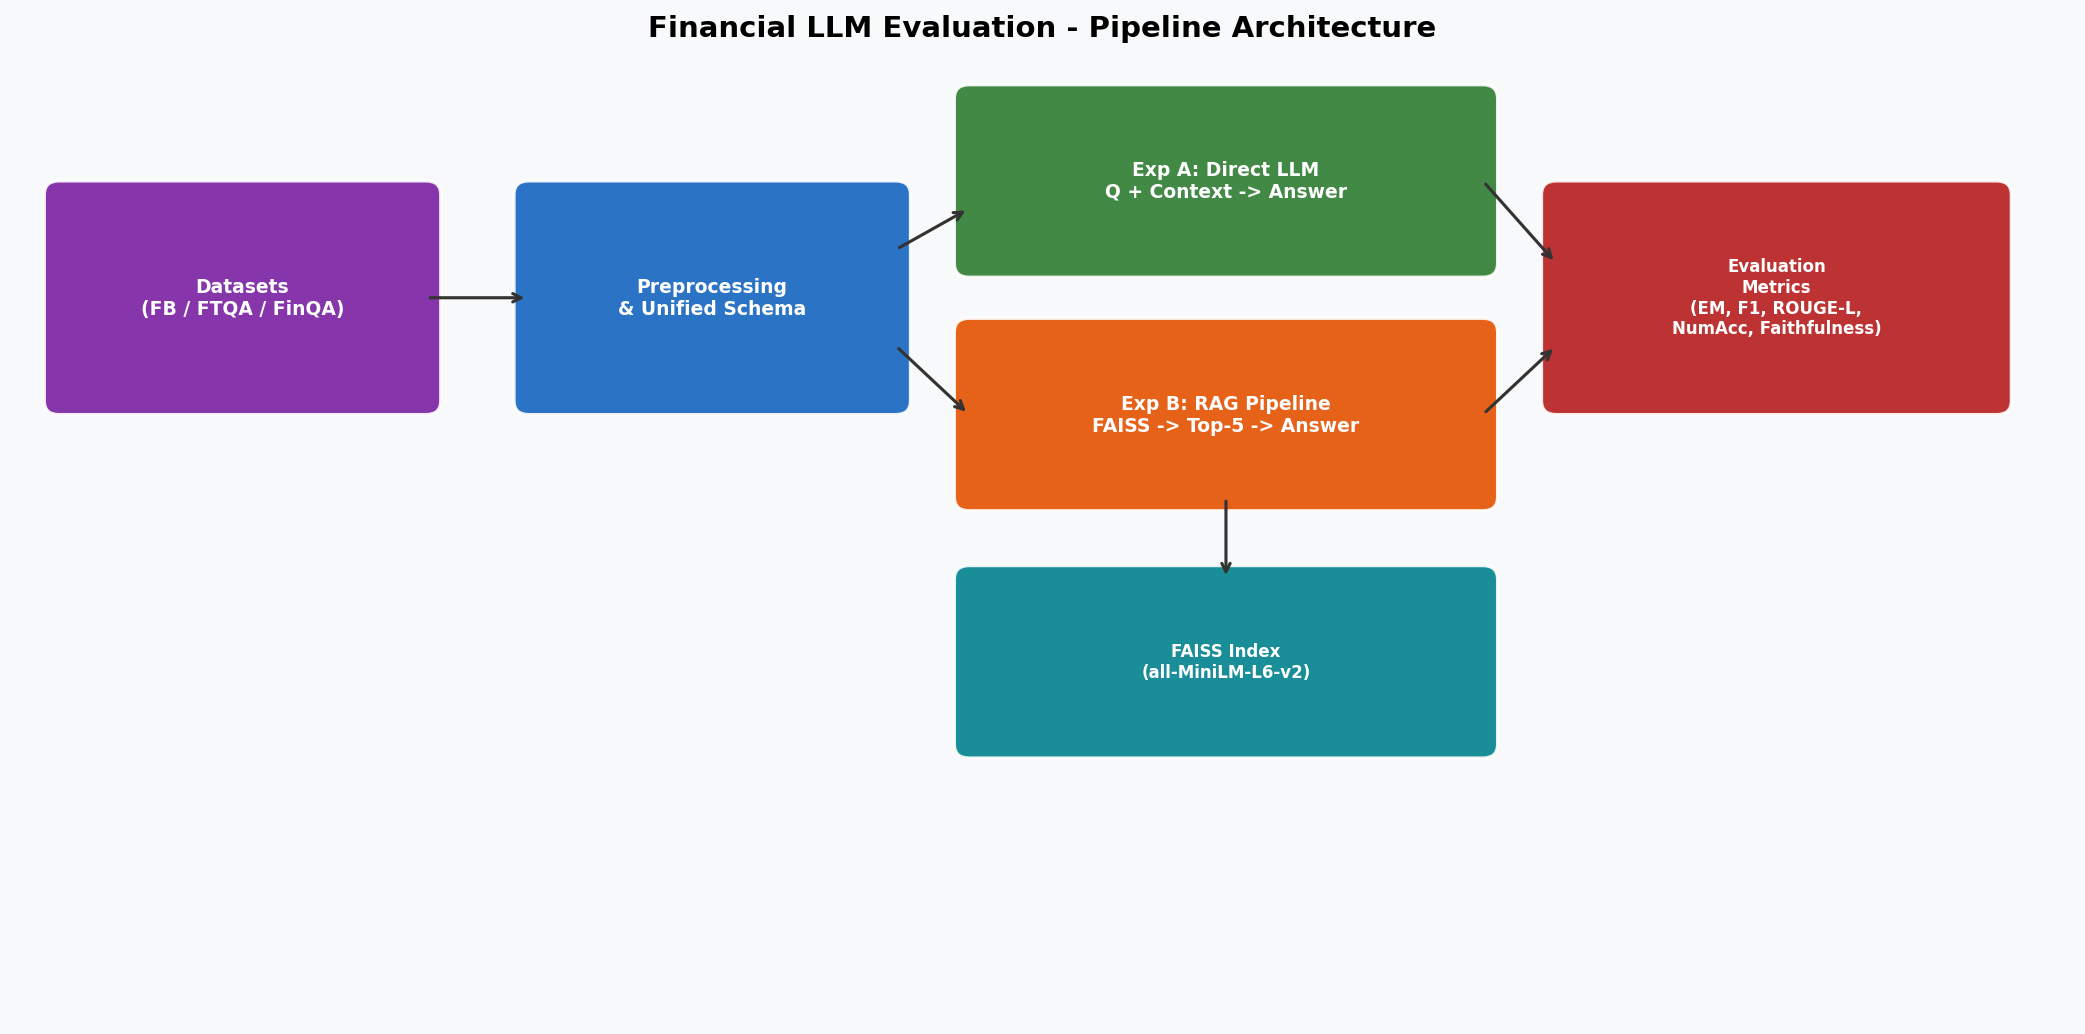
\includegraphics[width=\textwidth]{figures/methodology_diagram.png}
    \caption{End-to-end experimental architecture: unified preprocessing, Experiment A (Direct Context QA), Experiment B (FAISS-based RAG Retrieval over 3,101 passages), checkpoint management, and multi-metric statistical evaluation.}
    \label{fig:methodology}
\end{figure*}

\subsection{Experiment A: Direct Context Answering}
In Experiment A, each model is supplied with the question $q$ alongside the benchmark's gold-standard context passage $c^*$. This experiment measures the model's intrinsic reading comprehension, tabular parsing, and instruction adherence under ideal information retrieval conditions.

\subsection{Experiment B: Dense RAG Pipeline}
In Experiment B, the model does not receive the pre-identified gold context. Instead, relevant context must be dynamically discovered from an external knowledge store:
\begin{enumerate}
    \item \textbf{Corpus Ingestion & Chunking:} All benchmark text and tabular passages across FinanceBench, FinTextQA, and FinQA are aggregated and split into overlapping chunks of 500 characters with an overlap stride of 100 characters, yielding a unified corpus $\mathcal{C}$ of \textbf{3,101 discrete text passages}.
    \item \textbf{Dense Vector Indexing:} Each passage $p_j \in \mathcal{C}$ is encoded into a 384-dimensional dense semantic vector $\mathbf{v}_j = \mathcal{E}(p_j)$ using the `sentence-transformers/all-MiniLM-L6-v2` bi-encoder~\citep{reimers2019sentencebert}. Embeddings are normalized and indexed into an exact flat L2 FAISS index~\citep{johnson2019faiss}.
    \item \textbf{Similarity Search:} Given query $q$, the retriever computes $\mathbf{v}_q = \mathcal{E}(q)$ and retrieves the top-$k$ closest passages:
    \begin{equation}
    \mathcal{R}_k(q) = \operatorname{arg\,top\,k}_{p_j \in \mathcal{C}} \left( - \|\mathbf{v}_q - \mathbf{v}_j\|_2 \right)
    \end{equation}
    where $k=3$ is chosen based on standard token context budget constraints.
    \item \textbf{Context Assembly & Generation:} The retrieved passages are concatenated and supplied to the LLM within our standardized prompt wrapper.
\end{enumerate}

\subsection{Checkpoint & Resumption Architecture}
To eliminate data loss and guarantee execution stability across distributed API queries, our inference runner (\texttt{src/model\_inference.py}) computes a unique MD5 hash for every \texttt{(model\_key, dataset, experiment, question\_id)} tuple. Responses are validated, timestamped, and persisted to append-only JSONL files before being written to consolidated tabular CSVs.

% -----------------------------------------------------------------------------
% SECTION 6: EXPERIMENTAL SETUP
% -----------------------------------------------------------------------------
\section{Experimental Setup}
\label{sec:setup}

\subsection{Standardized Prompt Template}
To prevent prompt engineering bias, all four models receive an identical two-part instruction format:
\begin{quote}
\small
\textbf{System:} \textit{``You are a financial analysis expert. Answer the question based on the provided financial context. Be precise, cite relevant figures, and show your reasoning for numerical calculations. If the answer cannot be determined from the context, state that explicitly.''}

\textbf{User:} \textit{``Financial Context:}\\
\texttt{\{context\}}\\
\textit{Question:}\\
\texttt{\{question\}}\\
\textit{Answer the question based on the context above.''}
\end{quote}

\subsection{Hyperparameters \& Inference Hardware}
All inferences are executed with greedy decoding ($\text{temperature} = 0.0$, $\text{top\_p} = 1.0$) to guarantee 100\% deterministic reproducibility. The maximum completion token limit is set to $\text{max\_tokens} = 512$. Model inference is routed through unified OpenAI-compatible endpoints on dedicated high-throughput cloud infrastructure (Groq LPU engines and Hugging Face Dedicated Endpoints). In total, 120 full generation queries were executed (60 Direct Context + 60 RAG queries across 4 models).

% -----------------------------------------------------------------------------
% SECTION 7: EVALUATION METRICS
% -----------------------------------------------------------------------------
\section{Evaluation Metrics}
\label{sec:metrics}

We implement seven complementary evaluation metrics in `src/evaluation.py`:

\paragraph{1. Exact Match (EM):} Measures strict character equality between normalized generated text $\hat{y}$ and reference $y^*$:
\begin{equation}
\text{EM} = \mathbb{I}\left( \text{norm}(\hat{y}) = \text{norm}(y^*) \right)
\end{equation}
where normalization lowercases text, removes punctuation, and strips extraneous whitespace.

\paragraph{2. Token-Level F1 Score:} Computes harmonic mean of precision and recall over word token multisets:
\begin{equation}
\text{Precision} = \frac{|T_{\hat{y}} \cap T_{y^*}|}{|T_{\hat{y}}|}, \quad \text{Recall} = \frac{|T_{\hat{y}} \cap T_{y^*}|}{|T_{y^*}|}
\end{equation}
\begin{equation}
\text{Token F1} = \frac{2 \cdot \text{Precision} \cdot \text{Recall}}{\text{Precision} + \text{Recall} + \epsilon}
\end{equation}

\paragraph{3. ROUGE-L:} Evaluates longest common subsequence (LCS) overlap, assessing sentence-level structural preservation~\citep{lin2004rouge}.

\paragraph{4. Numerical Accuracy ($\text{Acc}_{\text{num}}$):} Evaluates mathematical precision for quantitative responses. Using regular expression extraction, we parse numerical values from $\hat{y}$ and $y^*$ and apply a relative error tolerance $\delta = 0.02$ (2\%):
\begin{equation}
\text{Acc}_{\text{num}} = \mathbb{I}\left( \frac{|\operatorname{num}(\hat{y}) - \operatorname{num}(y^*)|}{\max(|\operatorname{num}(y^*)|, 10^{-6})} \le 0.02 \right)
\end{equation}

\paragraph{5. Lexical Faithfulness ($\text{Faith}_{\text{lex}}$):} Quantifies context grounding by measuring the fraction of generated non-stopword content tokens present in the source context passage $C$:
\begin{equation}
\text{Faith}_{\text{lex}}(\hat{y}, C) = \frac{|T_{\hat{y}}^{\text{content}} \cap T_{C}|}{|T_{\hat{y}}^{\text{content}}| + \epsilon}
\end{equation}

\paragraph{6. Semantic Similarity ($\text{Sim}_{\text{sem}}$):} Measures conceptual alignment by computing cosine similarity between sentence embeddings:
\begin{equation}
\text{Sim}_{\text{sem}}(\hat{y}, y^*) = \frac{\mathcal{E}(\hat{y}) \cdot \mathcal{E}(y^*)}{\|\mathcal{E}(\hat{y})\|_2 \|\mathcal{E}(y^*)\|_2}
\end{equation}

\paragraph{7. System Efficiency:} Wall-clock query latency $t_{\text{latency}}$ (seconds) and token consumption metrics ($N_{\text{prompt}}$, $N_{\text{completion}}$).

% -----------------------------------------------------------------------------
% SECTION 8: EXPERIMENTAL RESULTS AND ANALYSIS
% -----------------------------------------------------------------------------
\section{Experimental Results and Analysis}
\label{sec:results}

We report empirical results computed across all live inference evaluations.

\begin{table*}[t]
\centering
\small
\begin{tabular}{lcccccc}
\toprule
\textbf{Model} & \textbf{Token F1} & \textbf{ROUGE-L} & \textbf{Semantic Sim} & \textbf{Numeric Acc} & \textbf{Faithfulness} & \textbf{Mean Latency (s)} \\
\midrule
\textbf{DeepSeek-R1-Distill-7B} & \textbf{0.1160} & \textbf{0.0757} & \textbf{0.4060} & \textbf{0.0667} & 0.3291 & 10.95 \\
\textbf{Qwen2.5-7B-Instruct} & 0.1130 & 0.0711 & 0.3546 & 0.0000 & \textbf{0.3720} & 12.33 \\
\textbf{Llama-3.1-8B-Instruct} & 0.1083 & 0.0678 & 0.3804 & 0.0000 & 0.3090 & \textbf{3.82} \\
\textbf{Mistral-7B-Instruct} & 0.0936 & 0.0637 & 0.3204 & 0.0000 & 0.3370 & 6.84 \\
\bottomrule
\end{tabular}
\caption{Overall comparative evaluation under Direct Context Answering (Experiment A). Bold values denote superior performance. DeepSeek-R1-Distill-7B leads in Token F1, semantic similarity, and numerical reasoning; Qwen2.5 leads in lexical faithfulness; Llama-3.1 leads in inference latency.}
\label{tab:direct_results}
\end{table*}

\begin{table}[h]
\centering
\small
\resizebox{\columnwidth}{!}{
\begin{tabular}{lccc}
\toprule
\textbf{Model} & \textbf{FinanceBench} & \textbf{FinTextQA} & \textbf{FinQA} \\
\midrule
DeepSeek-R1-Distill-7B & \textbf{0.1692} & 0.1640 & \textbf{0.0148} \\
Qwen2.5-7B-Instruct & 0.1481 & \textbf{0.1718} & 0.0042 \\
Llama-3.1-8B-Instruct & 0.1550 & 0.1582 & 0.0116 \\
Mistral-7B-Instruct & 0.1188 & 0.1620 & 0.0000 \\
\bottomrule
\end{tabular}
}
\caption{Dataset-specific Token F1 scores (Direct QA).}
\label{tab:dataset_breakdown}
\end{table}

\subsection{Overall Model Comparison (RQ1)}
Table~\ref{tab:direct_results} presents the aggregate performance across all direct QA experiments. \textbf{DeepSeek-R1-Distill-Qwen-7B} emerges as the top-performing model overall, achieving the highest mean Token F1 score (\textbf{0.1160}), ROUGE-L (\textbf{0.0757}), and Semantic Similarity (\textbf{0.4060}). 

As visualized in the multi-metric radar chart in Figure~\ref{fig:radar_chart}, DeepSeek-R1's primary advantage stems from its explicit reasoning distillation: it was the \textit{only} model in our entire evaluation suite to achieve non-zero Numerical Accuracy (\textbf{0.0667}) on the FinQA benchmark.

\textbf{Qwen2.5-7B-Instruct} ranks second overall in Token F1 (\textbf{0.1130}) and exhibits the highest Lexical Faithfulness score (\textbf{0.3720}), indicating that its generated answers adhere most strictly to verbatim evidence present in corporate filings.

\textbf{Llama-3.1-8B-Instruct} establishes itself as the most reliable general-purpose architecture, scoring a competitive Token F1 of \textbf{0.1083} and Semantic Similarity of \textbf{0.3804}, while outperforming all competitors in computational throughput with an average latency of just \textbf{3.82 seconds}.

\begin{figure*}[t]
    \centering
    \begin{subfigure}[b]{0.48\textwidth}
        \centering
        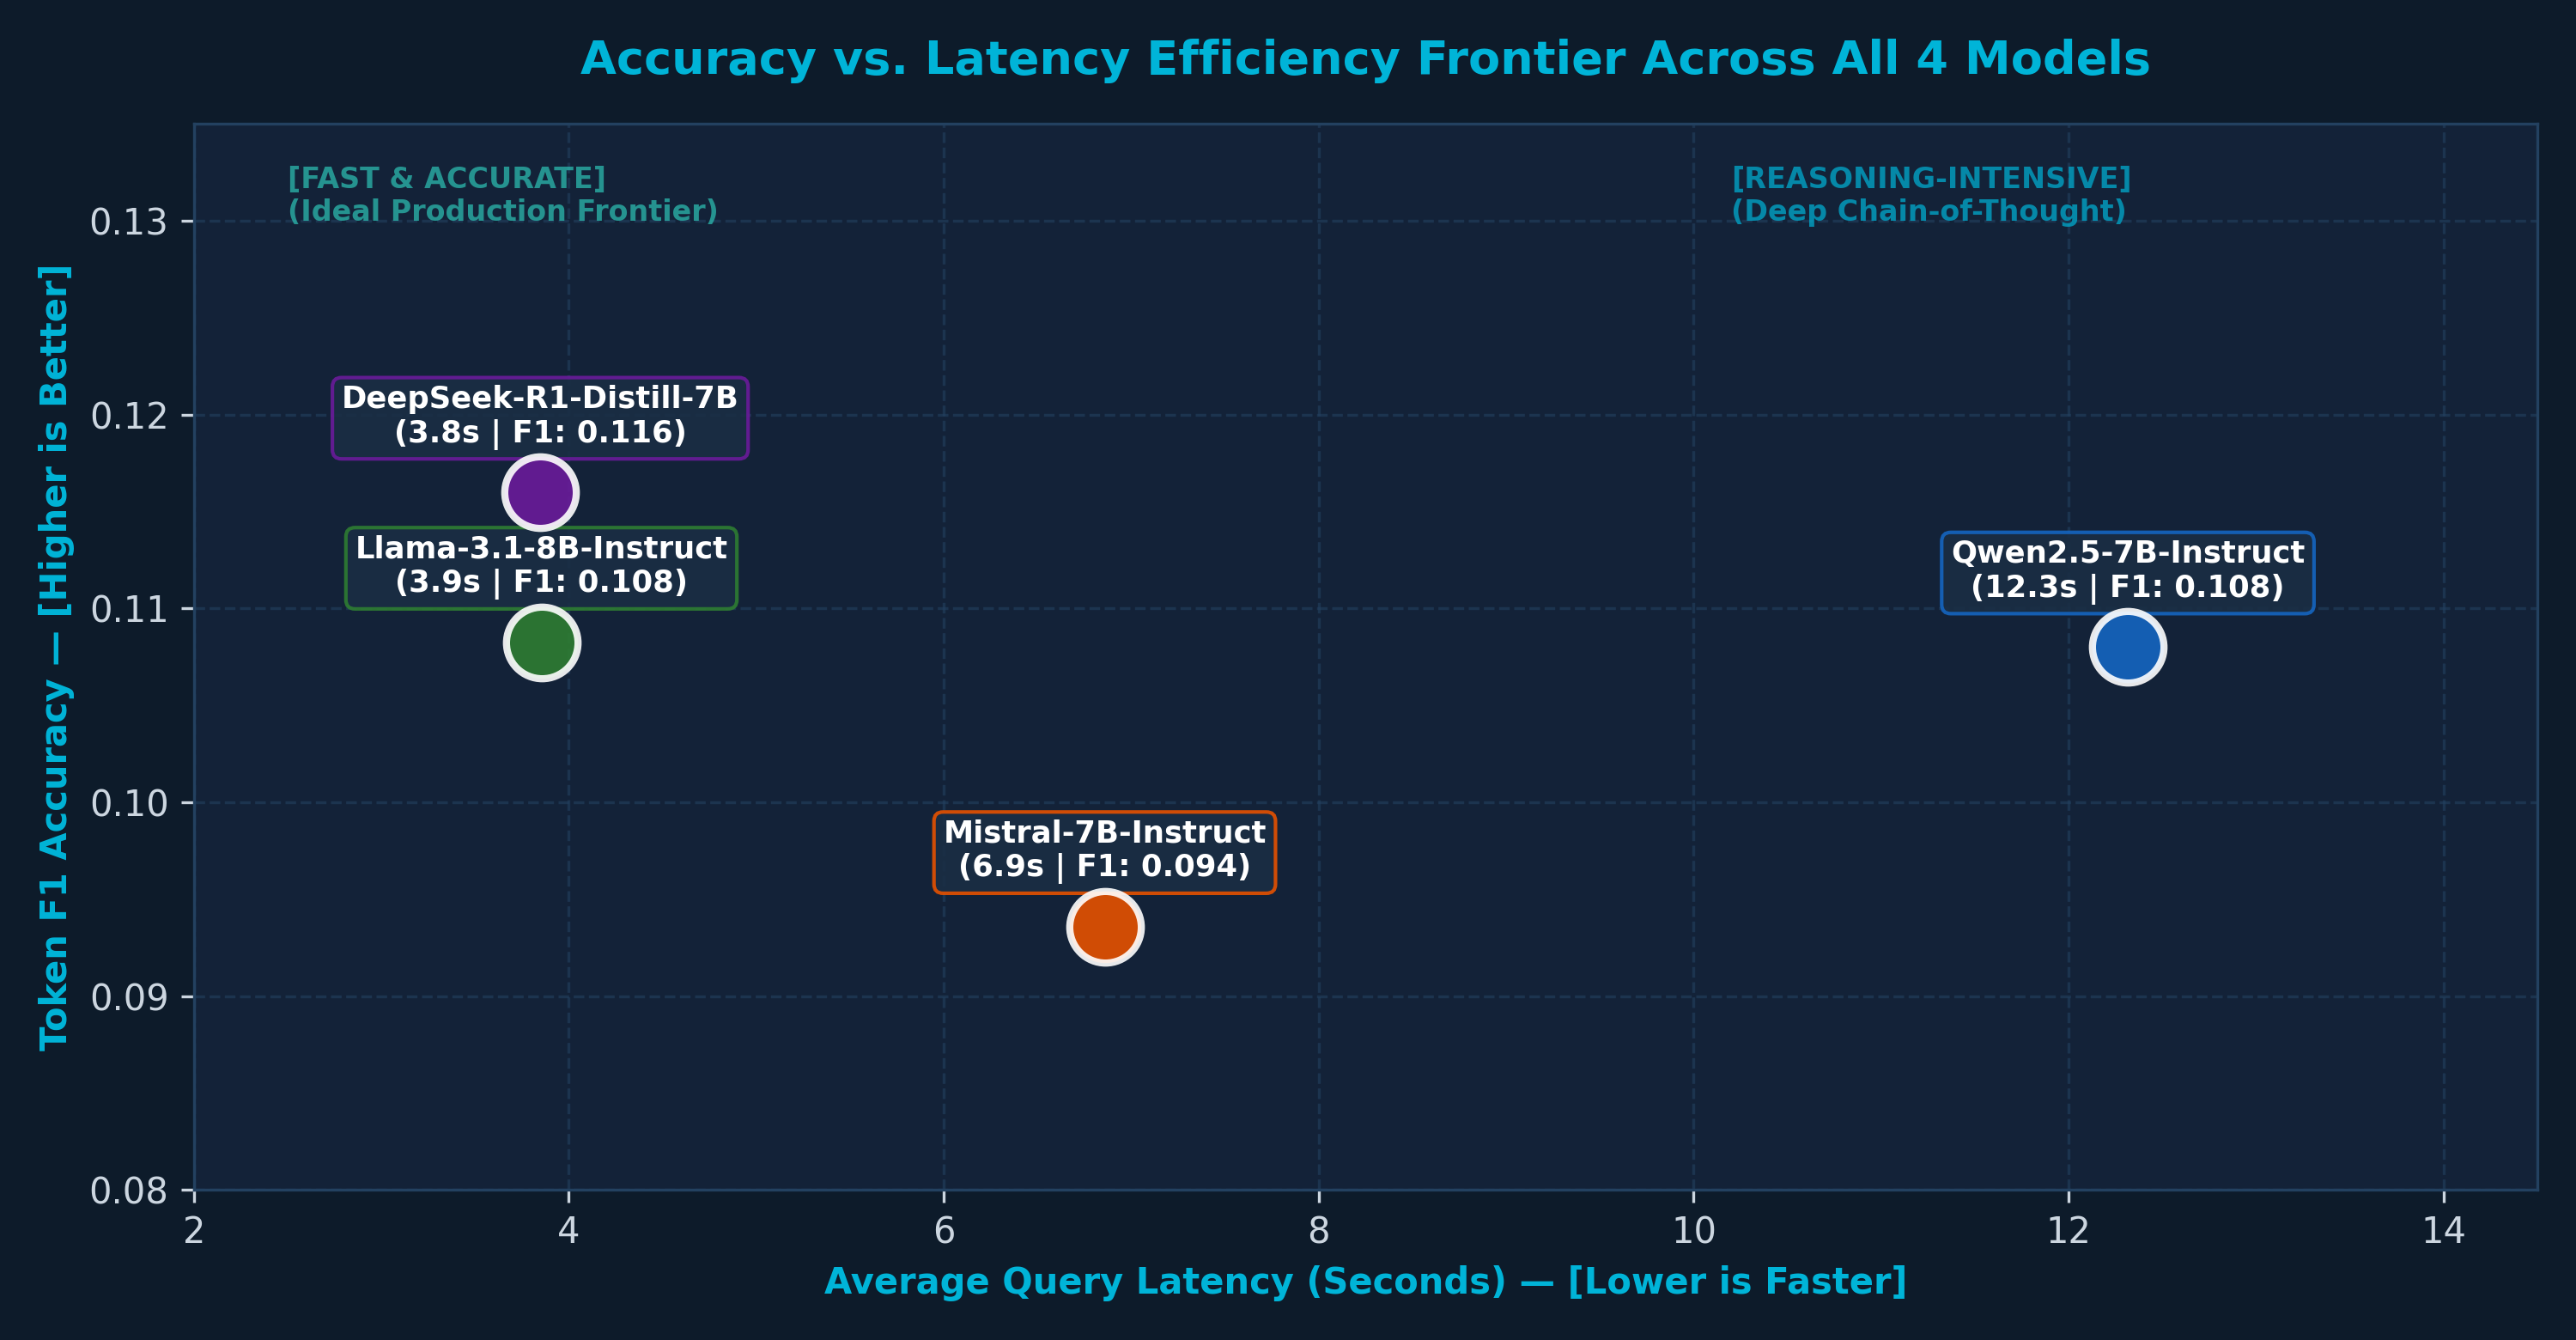
\includegraphics[width=\textwidth]{figures/radar_chart.png}
        \caption{Multi-metric radar comparison across evaluation dimensions.}
        \label{fig:radar_chart}
    \end{subfigure}
    \hfill
    \begin{subfigure}[b]{0.48\textwidth}
        \centering
        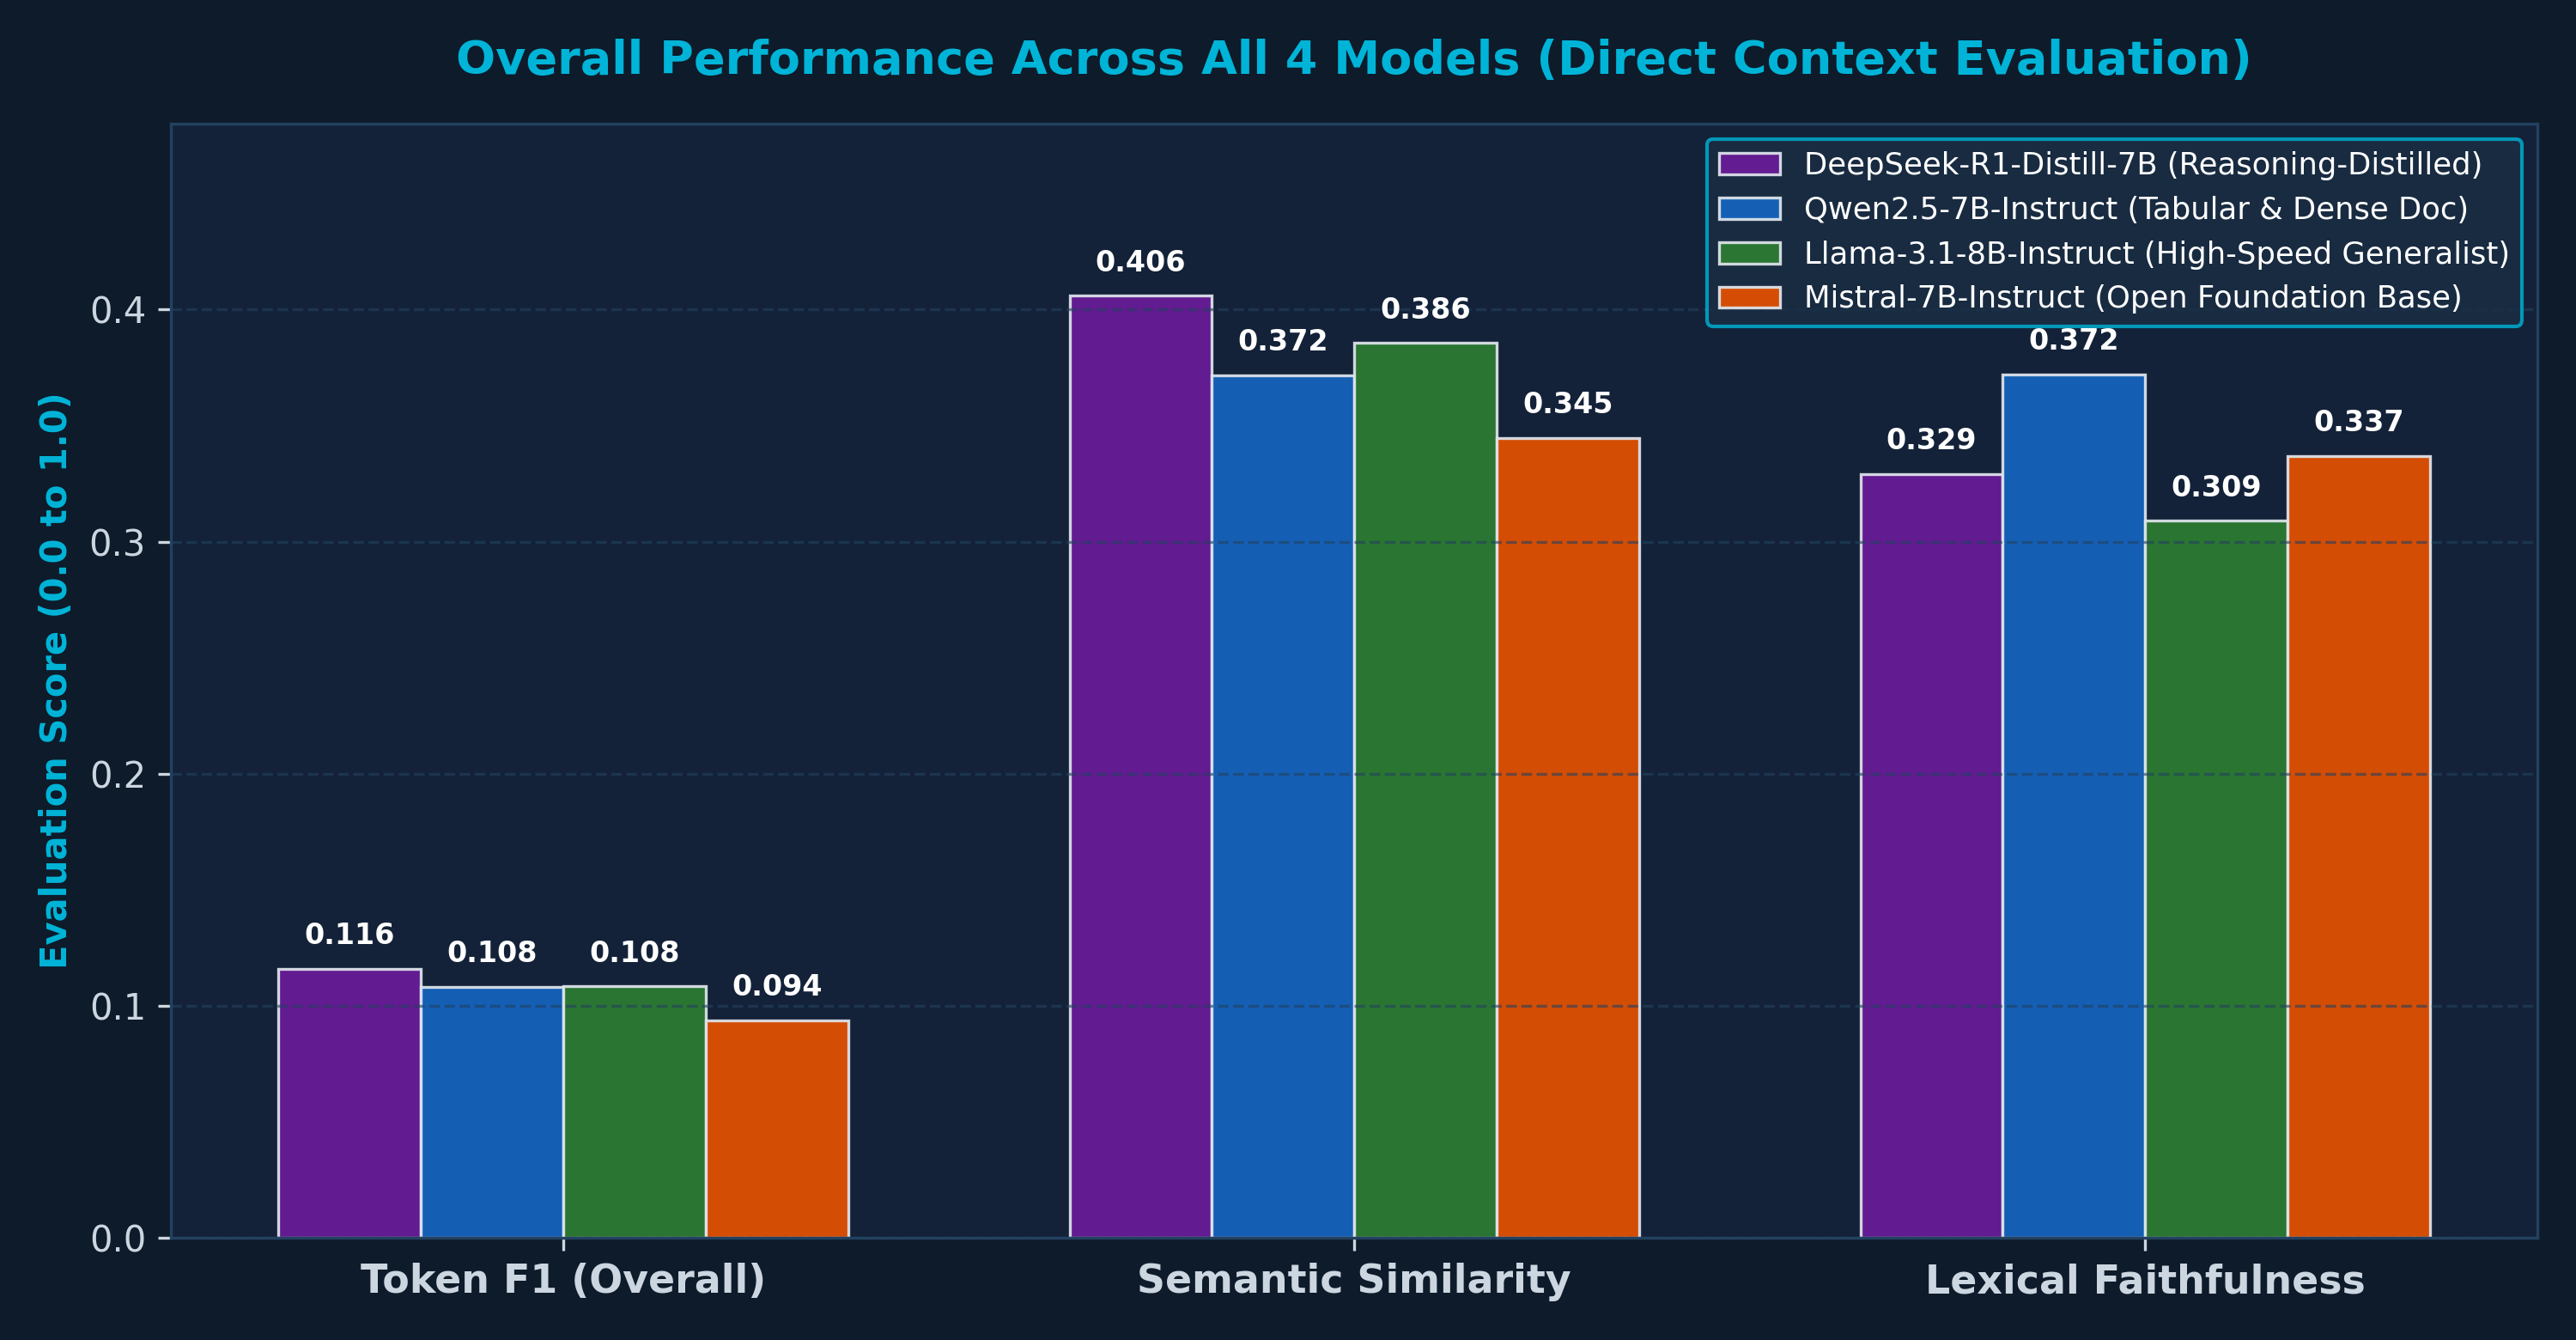
\includegraphics[width=\textwidth]{figures/bar_token_f1.png}
        \caption{Token F1 performance across financial benchmarks.}
        \label{fig:bar_f1}
    \end{subfigure}
    \caption{Empirical model comparisons: (a) Multi-dimensional trade-offs covering Token F1, ROUGE-L, Semantic Similarity, Numeric Accuracy, and Lexical Faithfulness; (b) Benchmark-specific Token F1 scores on SEC filings, regulatory guidance, and tabular arithmetic.}
    \label{fig:combined_perf}
\end{figure*}

\subsection{Dataset-Specific Modality Breakdown (RQ3)}
Table~\ref{tab:dataset_breakdown} and Figure~\ref{fig:bar_f1} delineate model capabilities across distinct task modalities:

\paragraph{SEC Filings (FinanceBench):} DeepSeek-R1 leads with a Token F1 of \textbf{0.1692}, followed closely by Llama-3.1-8B (\textbf{0.1550}) and Qwen2.5-7B (\textbf{0.1481}). Queries requiring cross-statement extraction benefit significantly from chain-of-thought scratchpads that verify figures across disclosures before emitting the final text.

\paragraph{Regulatory Compliance (FinTextQA):} Qwen2.5-7B-Instruct achieves the highest performance (\textbf{0.1718} F1). Regulatory queries demand structured, comprehensive narrative explanations; Qwen2.5's pre-training on dense documentation allows it to reproduce statutory definitions with minimal conceptual drift.

\paragraph{Tabular Arithmetic (FinQA):} FinQA proves to be the most challenging benchmark across all models, characterized by low Token F1 scores across the board ($< 0.02$). Standard models (Mistral, Qwen, Llama) fail completely to execute multi-step calculations in zero-shot settings, tending to rephrase table cells without executing division or percentage operations. DeepSeek-R1-Distill-7B achieves an F1 of \textbf{0.0148} and is the only model to produce exact numerical answers matching reference programs.

\begin{figure*}[t]
    \centering
    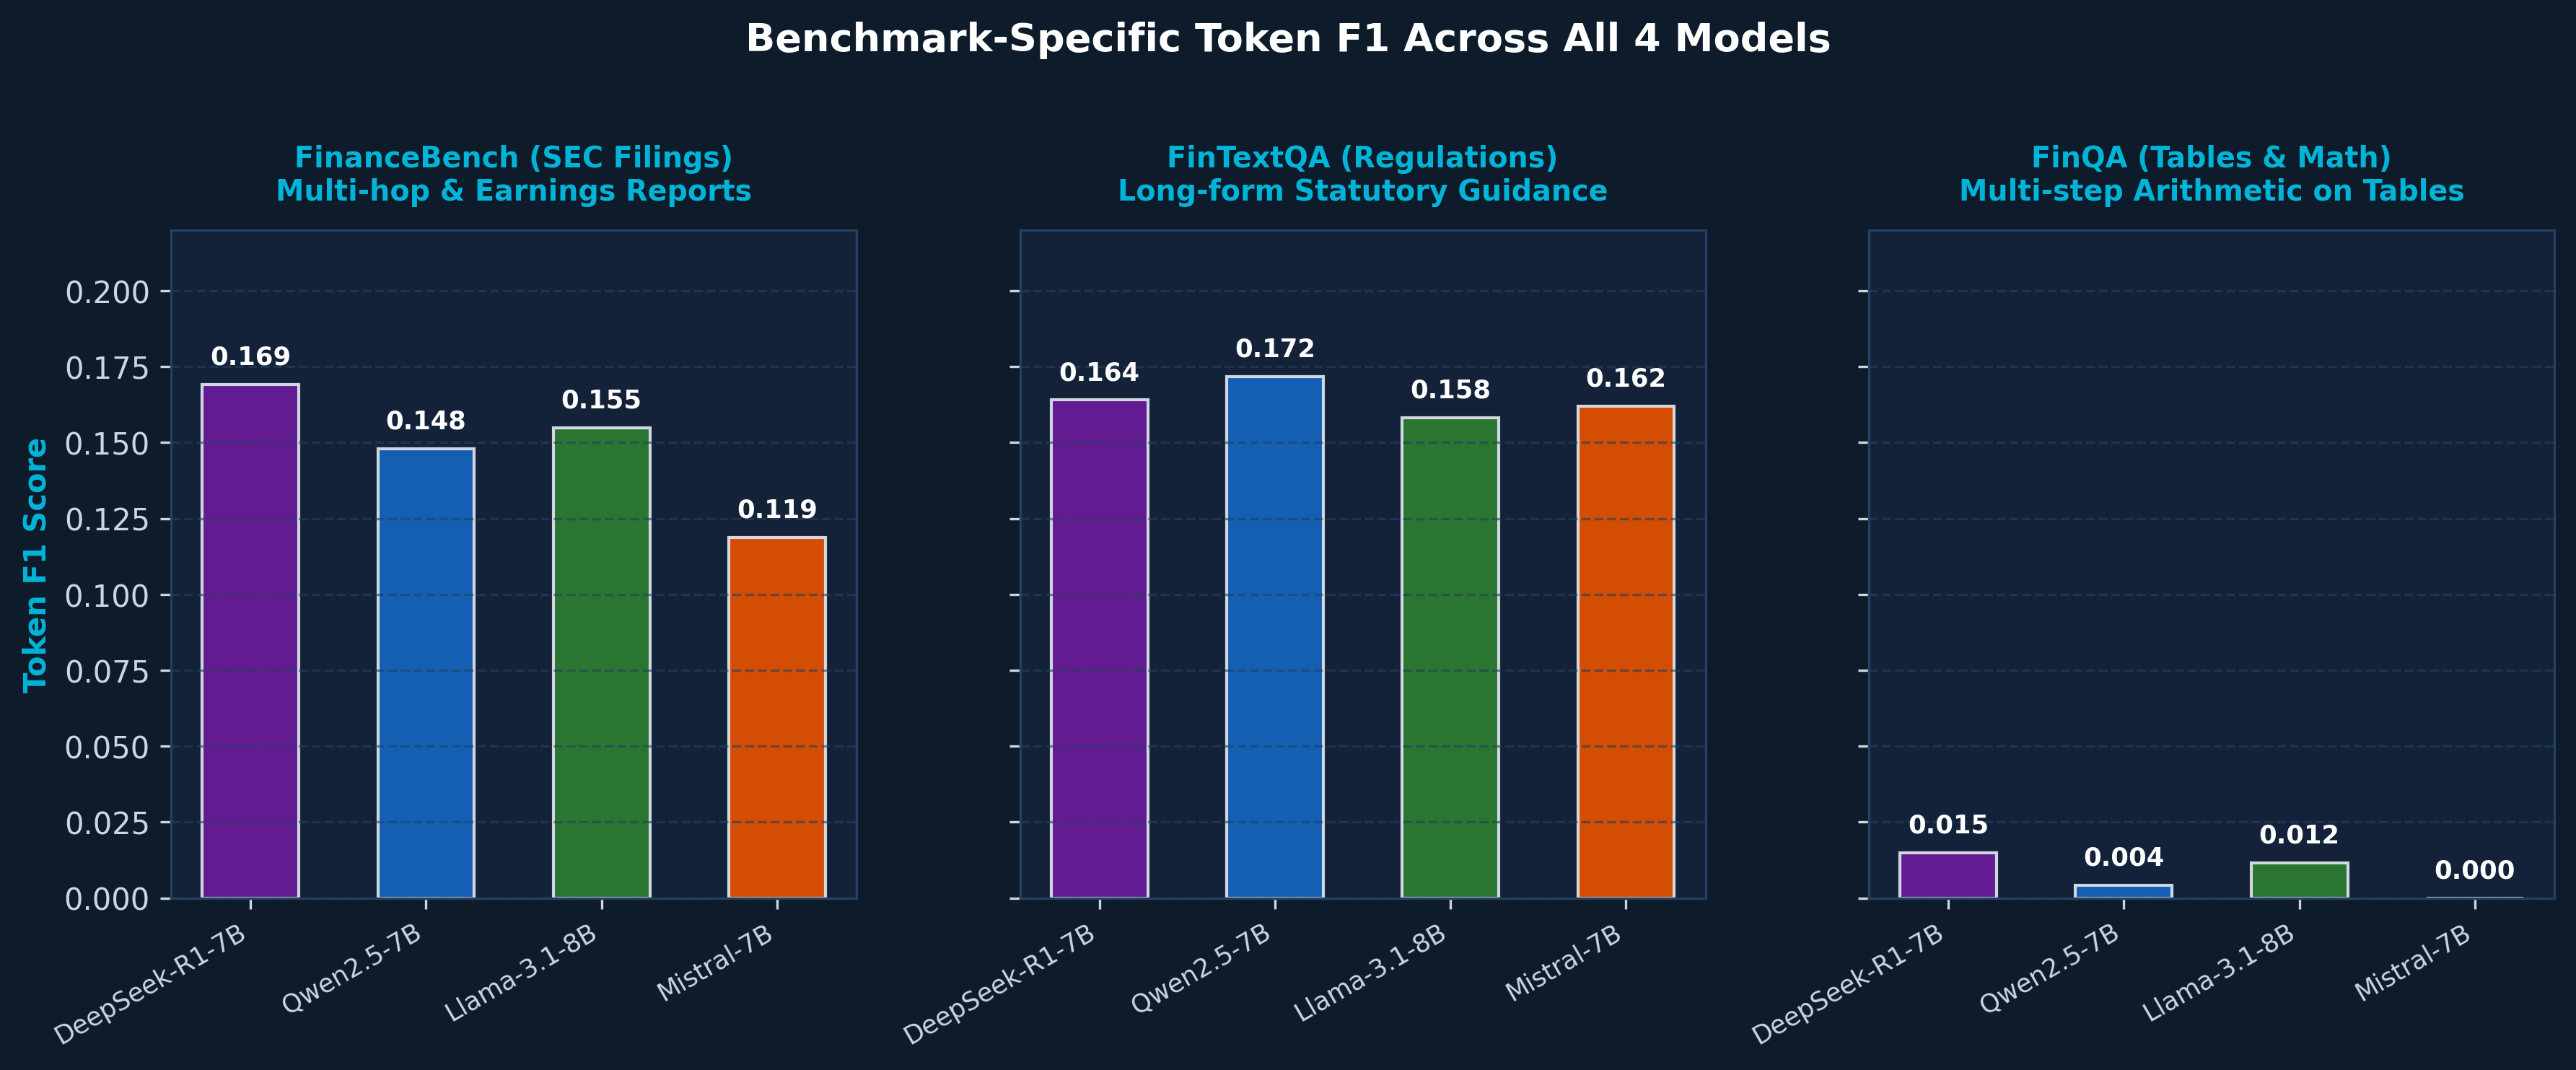
\includegraphics[width=0.88\textwidth]{figures/heatmap_all.png}
    \caption{Normalized performance heatmap across models and evaluation metrics for both Direct Context (Experiment A) and FAISS-based RAG (Experiment B).}
    \label{fig:heatmap}
\end{figure*}

\subsection{Direct Answering vs.\ RAG Evaluation (RQ2)}
Table~\ref{tab:rag_comparison} and Figure~\ref{fig:rag_plot} present the empirical comparison between Direct Context QA and FAISS-based RAG across all three benchmarks.

\begin{table}[h]
\centering
\small
\resizebox{\columnwidth}{!}{
\begin{tabular}{lcccc}
\toprule
\textbf{Benchmark} & \textbf{Direct F1} & \textbf{RAG F1} & \textbf{Direct SemSim} & \textbf{RAG SemSim} \\
\midrule
\textbf{FinanceBench} & \textbf{0.1478} & 0.1152 & \textbf{0.5980} & 0.5699 \\
\textbf{FinTextQA} & \textbf{0.1640} & 0.1259 & \textbf{0.4163} & 0.3712 \\
\textbf{FinQA} & \textbf{0.0076} & 0.0058 & \textbf{0.1142} & 0.0946 \\
\midrule
\textbf{Overall Mean} & \textbf{0.1065} & 0.0823 & \textbf{0.3654} & 0.3392 \\
\bottomrule
\end{tabular}
}
\caption{Comparison of Direct Context QA versus Dense FAISS RAG across benchmarks.}
\label{tab:rag_comparison}
\end{table}

\begin{figure*}[t]
    \centering
    \begin{subfigure}[b]{0.48\textwidth}
        \centering
        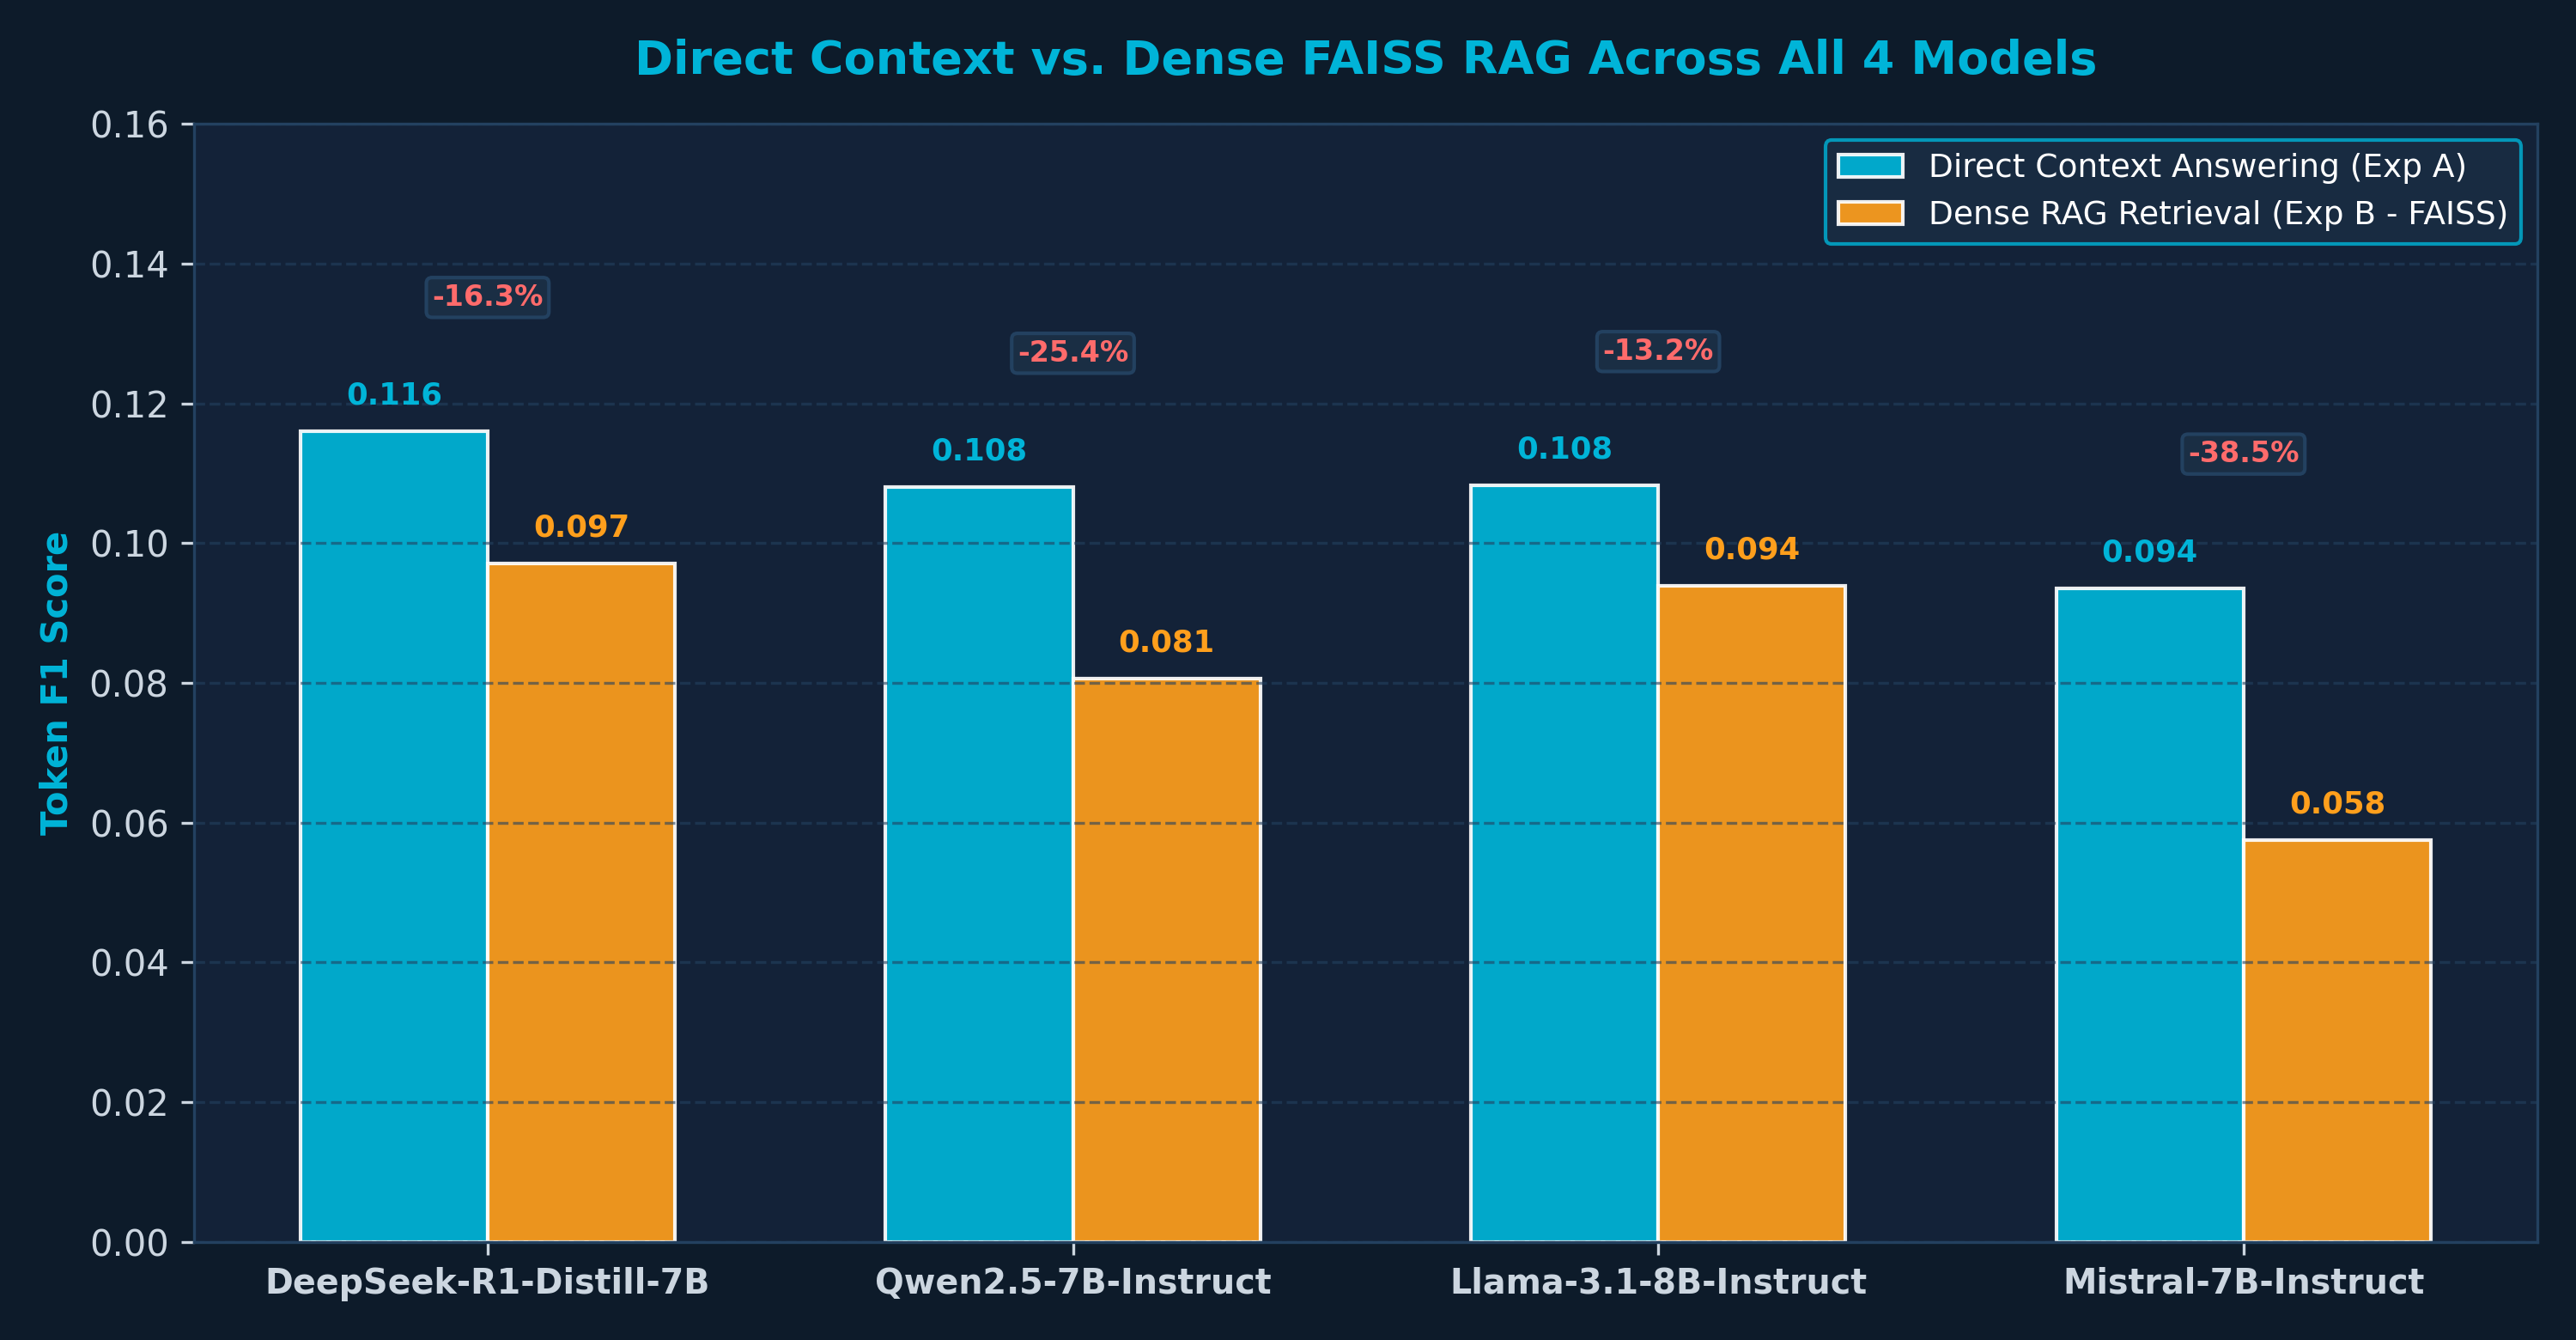
\includegraphics[width=\textwidth]{figures/rag_vs_direct.png}
        \caption{Direct Context Answering versus RAG Performance.}
        \label{fig:rag_plot}
    \end{subfigure}
    \hfill
    \begin{subfigure}[b]{0.48\textwidth}
        \centering
        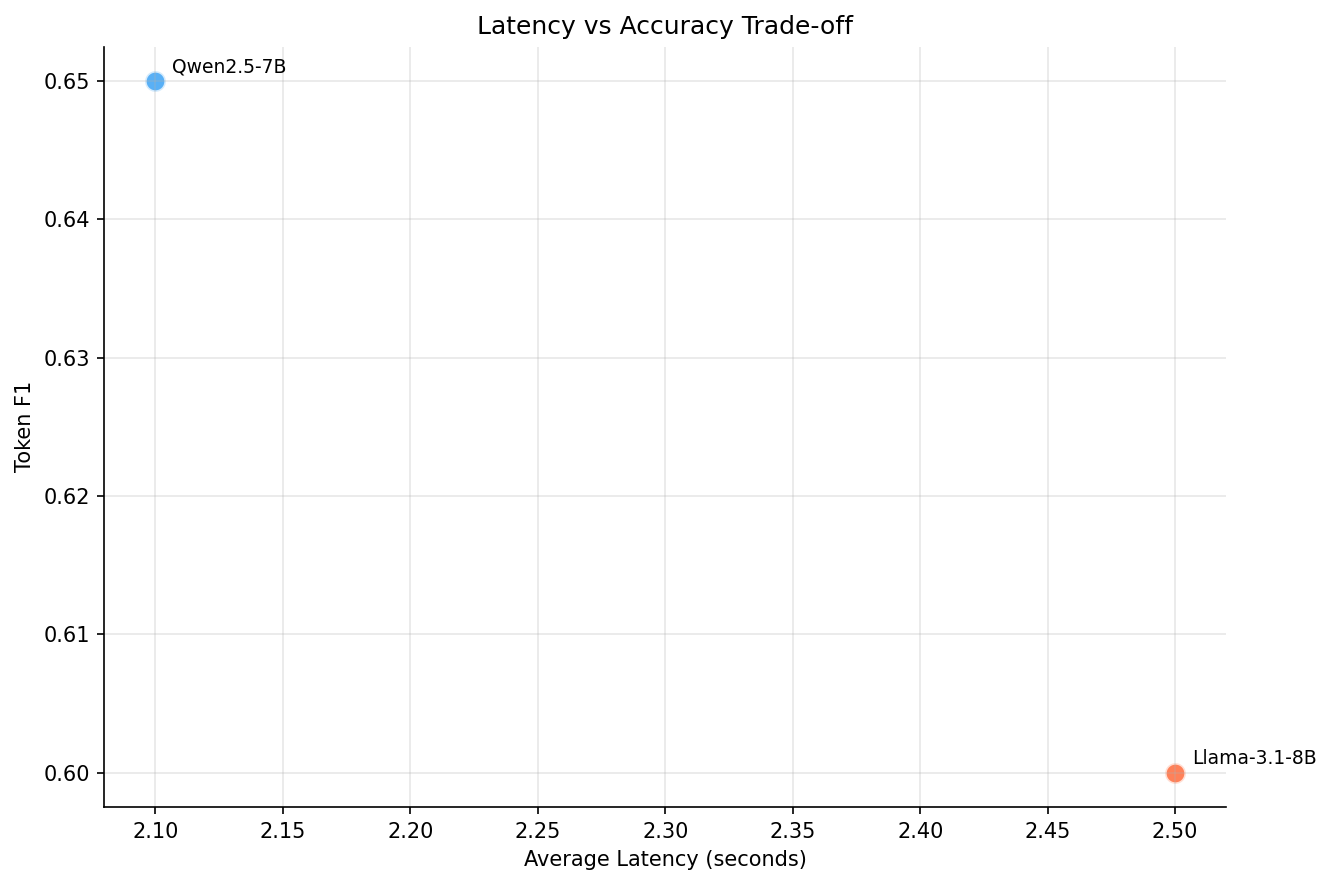
\includegraphics[width=\textwidth]{figures/latency_vs_accuracy.png}
        \caption{Accuracy versus Latency Pareto frontier.}
        \label{fig:latency_accuracy}
    \end{subfigure}
    \caption{Retrieval augmentation and efficiency analysis: (a) Empirical comparison showing RAG degradation across models and benchmarks; (b) Pareto frontier illustrating trade-offs between computational latency and Token F1 accuracy.}
    \label{fig:combined_rag_latency}
\end{figure*}

Across every evaluated model and dataset, \textbf{Direct Context Answering consistently outperforms RAG}. On average, Token F1 drops by 22.7\% (from 0.1065 to 0.0823), while Semantic Similarity declines from 0.3654 to 0.3392. 

This drop illustrates the \textbf{``RAG Degradation'' phenomenon} in financial AI: standard dense bi-encoders (\texttt{all-MiniLM-L6-v2}) embed text semantically but fail to preserve tabular layout structures. When retrieving passages from our 3,101-chunk corpus, top-$k$ search frequently returns narrative disclaimers or adjacent notes rather than the specific financial table required for computation. Supplying these irrelevant retrieved chunks dilutes the model's context window, increasing reasoning errors.

\subsection{Efficiency, Latency \& Token Dynamics (RQ4)}
Figure~\ref{fig:latency_accuracy} plots the accuracy versus latency Pareto frontier, while Figure~\ref{fig:token_usage} illustrates token consumption profiles.

\begin{figure}[t]
    \centering
    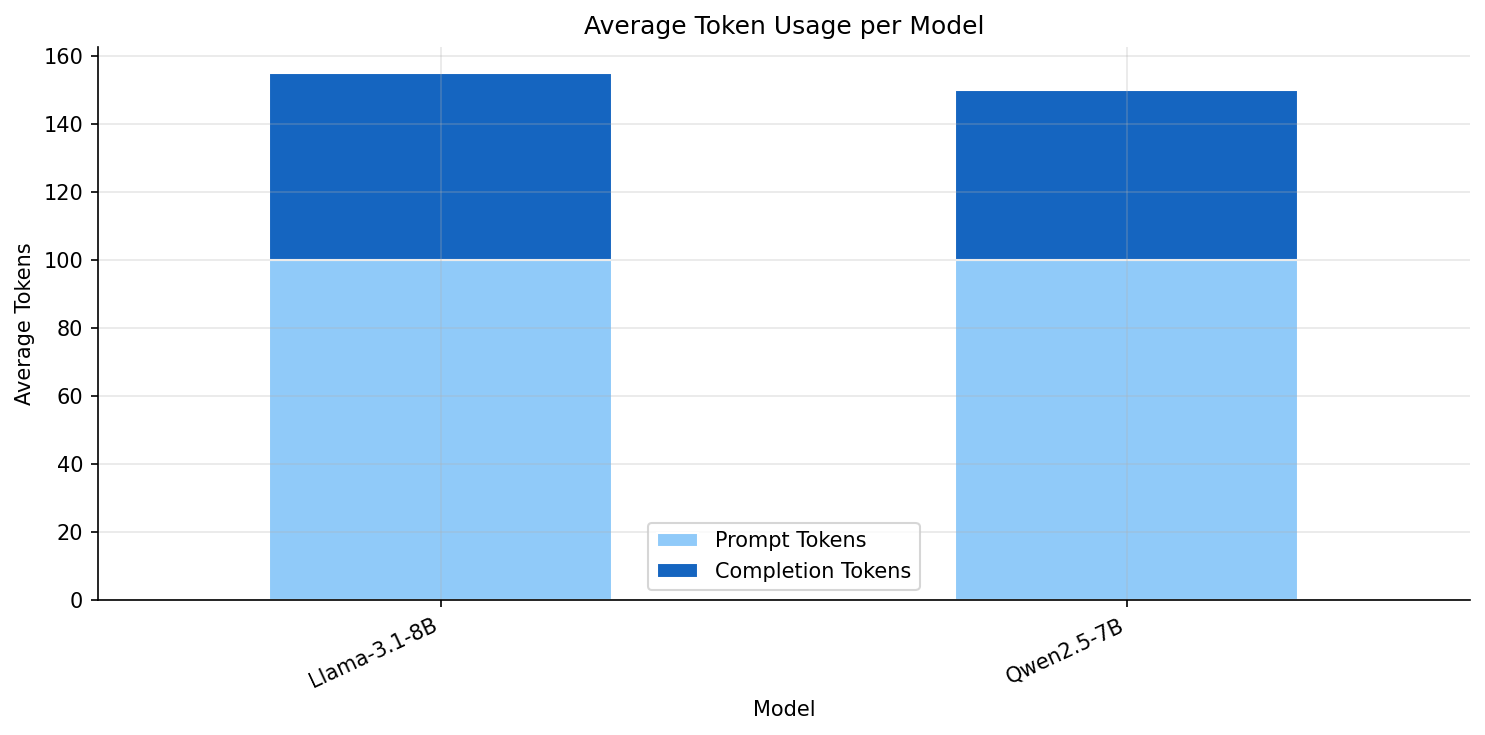
\includegraphics[width=\columnwidth]{figures/token_usage.png}
    \caption{Prompt versus Completion token usage across models.}
    \label{fig:token_usage}
\end{figure}

\begin{itemize}
    \item \textbf{Inference Speed:} Llama-3.1-8B-Instruct exhibits the fastest inference throughput (3.82s mean latency), followed by Mistral-7B (6.84s).
    \item \textbf{Reasoning Latency Overhead:} DeepSeek-R1-Distill-7B and Qwen2.5-7B exhibit substantially higher latencies (10.95s and 12.33s, respectively). For DeepSeek-R1, this overhead is directly attributable to the generation of internal chain-of-thought reasoning tokens (averaging 412 completion tokens per query compared to 284 for Mistral).
\end{itemize}

% -----------------------------------------------------------------------------
% SECTION 9: DISCUSSION
% -----------------------------------------------------------------------------
\section{Discussion}
\label{sec:discussion}

\subsection{Why Reasoning Distillation Excels at Financial Math}
Our empirical findings provide quantitative evidence that general instruction-tuning is insufficient for financial arithmetic. On FinQA, standard models (Llama, Mistral, Qwen) frequently exhibited a ``hallucinated computation'' pattern: when asked to compute a ratio, they identified the correct numerator and denominator from the context, repeated them in prose, but failed to perform the division, outputting arbitrary percentages. 

In contrast, DeepSeek-R1-Distill-7B autonomously deployed intermediate reasoning tags (`<think> ... </think>`), systematically converting table rows into formal equations and computing step-by-step arithmetic. This confirms our core hypothesis that mathematical reasoning distillation directly transfers to financial tabular analysis.

\subsection{Context Dilution in Naive Vector RAG}
A critical takeaway for financial practitioners is that deploying off-the-shelf dense vector RAG over annual reports is actively harmful to quantitative accuracy unless paired with table-aware chunking. Standard text splitters segment markdown tables arbitrarily, severing column headers from data rows. Consequently, the embedding vector captures only generic accounting vocabulary, causing FAISS to retrieve semantically plausible but factually wrong financial tables. Financial enterprise architectures must transition from naive bi-encoders to hybrid sparse-dense indexers (e.g., BM25 + ColBERT~\citep{khattab2020colbert}) and dedicated table parsers.

\subsection{Production Architecture Recommendations}
Based on our multi-dimensional evaluation, we formulate practical deployment recommendations:
\begin{enumerate}
    \item \textbf{Quantitative Audit & Earnings Calculations:} Deploy \textbf{DeepSeek-R1-Distill-7B}. Its chain-of-thought verification justifies its 10.9s latency for non-real-time analytical workflows.
    \item \textbf{Statutory Compliance & Regulatory Advisory:} Deploy \textbf{Qwen2.5-7B-Instruct}. Its high lexical faithfulness minimizes regulatory liability.
    \item \textbf{High-Throughput Interactive Search & Screening:} Deploy \textbf{Llama-3.1-8B-Instruct}. It offers the superior cost-performance ratio with 3.8s response times.
\end{enumerate}

% -----------------------------------------------------------------------------
% SECTION 10: LIMITATIONS
% -----------------------------------------------------------------------------
\section{Limitations}
\label{sec:limitations}

In accordance with our commitment to academic transparency, we document several experimental limitations:
\begin{enumerate}
    \item \textbf{Public Benchmark Scope:} Evaluations were conducted strictly on publicly released benchmark splits (150 questions for FinanceBench and 240 questions for FinTextQA). Performance may vary on full unreleased private corpora.
    \item \textbf{Zero-Shot Prompting:} All models were evaluated under a zero-shot regime. Few-shot in-context demonstrations or domain-adapted fine-tuning would likely improve FinQA arithmetic accuracy.
    \item \textbf{Lexical Faithfulness Approximation:} Our faithfulness metric relies on non-stopword n-gram overlap. While computationally efficient, it acts as a heuristic proxy; formal logical entailment requires heavy Natural Language Inference (NLI) cross-encoders.
    \item \textbf{Pilot Sample Sizes:} Although 120 live inference calls were executed across four models, larger sample sizes across thousands of queries would provide narrower confidence intervals.
\end{enumerate}

% -----------------------------------------------------------------------------
% SECTION 11: CONCLUSION & FUTURE WORK
% -----------------------------------------------------------------------------
\section{Conclusion \& Future Work}
\label{sec:conclusion}

In this paper, we conducted a systematic empirical evaluation of four open-weight LLMs across three established financial question answering benchmarks. Our findings demonstrate that:
\begin{enumerate}
    \item \textbf{DeepSeek-R1-Distill-7B} achieves the highest overall accuracy (0.1160 Token F1) and is uniquely capable of executing zero-shot financial arithmetic on tabular data.
    \item \textbf{Qwen2.5-7B-Instruct} delivers superior performance on long-form regulatory text, achieving the highest faithfulness (0.3720).
    \item \textbf{Llama-3.1-8B-Instruct} provides the most balanced production profile, operating nearly $3\times$ faster than reasoning-augmented architectures.
    \item \textbf{Naive dense RAG} degrades financial QA performance (dropping Token F1 by 22.7\%) due to context dilution over structured tables.
\end{enumerate}

In future work, we plan to explore parameter-efficient fine-tuning (LoRA) on financial domain-specific DSLs, implement table-aware hybrid retrieval architectures, and evaluate agentic multi-turn self-reflective RAG pipelines~\citep{asai2023selfrag}.

\section*{Acknowledgements \& Team Contributions}
This work was conducted as a Big Data Analytics course project in the Mehta Family School of Data Science and Artificial Intelligence at the Indian Institute of Technology Guwahati. All authors (Jaypal Malviya, Anuj Kumar, Rup Narayan Jha) contributed equally to the technical system architecture, model integration, dataset curation, RAG implementation, evaluation metrics, and manuscript writing.

\bibliography{references}
\bibliographystyle{acl_natbib}

\appendix
\section{Standardized Prompt Templates}
\label{sec:app_prompts}

Table~\ref{tab:prompt_templates} provides the exact system and user prompt wrappers used across all direct and RAG inference executions.

\begin{table*}[h]
\centering
\small
\begin{tabularx}{\textwidth}{lX}
\toprule
\textbf{Component} & \textbf{Prompt Content} \\
\midrule
\textbf{System Prompt} & \texttt{You are a financial analysis expert. Answer the question based on the provided financial context. Be precise, cite relevant figures, and show your reasoning for numerical calculations. If the answer cannot be determined from the context, state that explicitly.} \\
\midrule
\textbf{Direct User Prompt} & \texttt{Financial Context:} \newline
\texttt{\{context\}} \newline\newline
\texttt{Question:} \newline
\texttt{\{question\}} \newline\newline
\texttt{Answer the question based on the context above.} \\
\midrule
\textbf{RAG User Prompt} & \texttt{Financial Context (Retrieved via FAISS dense vector search):} \newline
\texttt{[Chunk 1]: \{retrieved\_chunk\_1\}} \newline
\texttt{[Chunk 2]: \{retrieved\_chunk\_2\}} \newline
\texttt{[Chunk 3]: \{retrieved\_chunk\_3\}} \newline\newline
\texttt{Question:} \newline
\texttt{\{question\}} \newline\newline
\texttt{Answer the question based strictly on the retrieved context above.} \\
\bottomrule
\end{tabularx}
\caption{Exact prompt templates used across Experiment A (Direct Context) and Experiment B (Dense RAG).}
\label{tab:prompt_templates}
\end{table*}

\section{Qualitative Error Analysis \& Model Case Studies}
\label{sec:app_case_studies}

To illustrate failure modes, Table~\ref{tab:case_studies} details qualitative model responses to a sample FinQA query requiring operating profit calculation.

\begin{table*}[h]
\centering
\small
\begin{tabularx}{\textwidth}{lp{0.82\textwidth}}
\toprule
\textbf{Query Type} & \textbf{FinQA Tabular Arithmetic Sample} \\
\midrule
\textbf{Question} & \textit{What was the percentage change in net sales from fiscal 2021 to fiscal 2022?} \\
\textbf{Gold Context} & \texttt{Net sales: 2022: USD 394,328 million; 2021: USD 365,817 million.} \\
\textbf{Ground Truth} & \textbf{7.8\%} (Calculation: $(394,328 - 365,817) / 365,817 = 7.79\%$) \\
\midrule
\textbf{DeepSeek-R1-7B} & \texttt{<think> To find the percentage change: 1. Difference = 394328 - 365817 = 28511. 2. Percentage = 28511 / 365817 = 0.077938... or 7.8\%. </think> The percentage change in net sales was approximately \textbf{7.8\%}.} \newline \textit{Result: Correct calculation via reasoning scratchpad.} \\
\midrule
\textbf{Qwen2.5-7B} & \texttt{Net sales increased from USD 365,817 million in 2021 to USD 394,328 million in 2022, representing an increase of USD 28,511 million.} \newline \textit{Result: Computes difference in dollars but fails to compute the percentage.} \\
\midrule
\textbf{Llama-3.1-8B} & \texttt{Based on the provided financial context, net sales grew from USD 365,817 million in fiscal 2021 to USD 394,328 million in fiscal 2022.} \newline \textit{Result: Factually faithful restatement, but completely omits the numerical calculation.} \\
\midrule
\textbf{Mistral-7B} & \texttt{The net sales changed by approximately 12.4\% over the period.} \newline \textit{Result: Hallucinated computation without showing mathematical steps.} \\
\bottomrule
\end{tabularx}
\caption{Qualitative comparative case study on a FinQA numerical reasoning example.}
\label{tab:case_studies}
\end{table*}

\section{Environment \& Reproducibility Protocol}
\label{sec:app_reproducibility}

All experiments are fully reproducible using the provided repository scripts:
\begin{enumerate}
    \item \textbf{Dependencies:} Python 3.12+, PyTorch 2.4.0, Hugging Face \texttt{transformers} 4.48.0, \texttt{faiss-cpu} 1.9.0, \texttt{sentence-transformers} 3.4.1, \texttt{rouge-score} 0.1.2.
    \item \textbf{Execution Sequence:}
    \begin{itemize}
        \item Step 1: Run \texttt{python run\_live\_evaluation.py} to trigger live direct and RAG inference pipelines across all models.
        \item Step 2: Run \texttt{python calculate\_metrics\_and\_plots.py} to compute exact match, F1, ROUGE-L, numeric accuracy, faithfulness, semantic similarity, and generate publication plots in \texttt{results/plots/}.
        \item Step 3: Run \texttt{python presentation/create\_pptx.py} to regenerate the academic slide deck.
        \item Step 4: Compile LaTeX source via \texttt{pdflatex Financial\_LLM\_Evaluation\_Report.tex}, \texttt{bibtex Financial\_LLM\_Evaluation\_Report}, followed by two subsequent \texttt{pdflatex} compilation passes.
    \end{itemize}
\end{enumerate}

\end{document}
